\documentclass[12pt,a4paper]{article}
\usepackage[utf8]{inputenc}
\usepackage[portuguese]{babel}
\usepackage[margin=2.5cm]{geometry}
\usepackage{amsmath}
\usepackage{amsfonts}
\usepackage{amssymb}
\usepackage{graphicx}
\usepackage{booktabs}
\usepackage{array}
\usepackage{longtable}
\usepackage{multirow}
\usepackage{xcolor}
\usepackage{enumitem}
\usepackage{hyperref}
\usepackage{fancyhdr}
\usepackage{titlesec}
\usepackage{tocloft}
\usepackage{float}

% Configuração do hyperref
\hypersetup{
    colorlinks=true,
    linkcolor=black,
    filecolor=magenta,
    urlcolor=cyan,
    citecolor=black,
    pdfborderstyle={/S/U/W 1}
}

% Configuração das seções
\titleformat{\section}{\Large\bfseries}{\thesection}{1em}{}
\titleformat{\subsection}{\large\bfseries}{\thesubsection}{1em}{}
\titleformat{\subsubsection}{\normalsize\bfseries}{\thesubsubsection}{1em}{}

% Configuração do cabeçalho e rodapé
\setlength{\headheight}{14.5pt}
\pagestyle{fancy}
\fancyhf{}
\fancyhead[L]{Plano de Projeto - Sistema Churrasco Entre Amigos}
\fancyfoot[C]{\thepage}

% Configuração do índice
\renewcommand{\cftsecleader}{\cftdotfill{\cftdotsep}}

\begin{document}

% Incluir a capa
%Capa------------------------------------------------------
\thispagestyle{empty}

\begin{minipage}[c]{0.3\textwidth}

\includegraphics[width=\textwidth]{unesp.png}
\end{minipage}
\hspace{10pt}
\begin{minipage}[c]{0.6\textwidth}
\uppercase{Universidade Estadual Paulista \\``Júlio de Mesquita Filho"}
\end{minipage}
\vspace{5mm}
\hrule
\vspace{5mm}
\begin{center}
    FCT - Faculdade de Ciências e Tecnologia\\
    DMC - Departamento de Matemática e Computação\\
    Bacharelado em Ciência da Computação\\
\end{center}

\vspace{1cm}

\begin{center}
    Engenharia de Software 2\\
    Projeto 3 - Sistema de Gestão de Churrascos Entre Amigos
\end{center}

\vspace{1.5cm}

\begin{center}
\Large\textbf{Plano de Projeto de Software}
\end{center}

\vspace{1cm}

Título do Sistema: 
\begin{center}
\Large\textbf{Sistema de Gestão de Churrascos Entre Amigos}\\[0.5cm]
\large\textbf{Pagamento Mensal e Controle de Despesas por Churrasco}
\end{center}

\vspace{2cm}

\begin{table}[H]
    \begin{tabular}{ll}
        Gerentes de Projeto: & Julio\\
                           & Ricardo\\
                           & Igor\\[1cm]
        SQA (Garantia de Qualidade): & Luiz\\
                                    & Sara\\[0.5cm]
        A\&P (Análise e Projeto): & Augusto\\
                                 & Pedro Coleta\\[0.5cm]
        COD (Codificação): & Guilherme Carrara\\
                          & Guilherme Digiorgi\\[1cm]
        Professor: & Prof. Dr. Rogério Garcia\\[1cm]
        Disciplina: & Engenharia de Software 2\\
    \end{tabular}
\end{table}

\vspace*{\fill}

\begin{center}
    Presidente Prudente, \today
\end{center}

\newpage


% Sumário
\tableofcontents
\newpage

% Conteúdo principal
\section{Resumo}

Este documento apresenta o plano completo para o desenvolvimento do Sistema de Gestão de Churrascos Entre Amigos, um software projetado para facilitar a organização, gestão financeira e coordenação de eventos sociais entre grupos de amigos.

O projeto será desenvolvido seguindo uma metodologia ágil com 4 sprints bem definidos, totalizando 86 dias úteis de desenvolvimento. O sistema contempla funcionalidades abrangentes desde o cadastro de usuários até a prestação de contas detalhada dos eventos.

\subsection{Objetivos Principais}
\begin{itemize}
    \item Automatizar o processo de organização de churrascos
    \item Facilitar o controle financeiro e divisão de despesas
    \item Implementar sistema de convites e confirmações automatizadas
    \item Proporcionar transparência na prestação de contas
    \item Ofertar cálculo automático de lista de compras
\end{itemize}

\subsection{Escopo do Projeto}
O sistema incluirá módulos para:
\begin{itemize}
    \item Gestão de usuários e autenticação
    \item Criação e gerenciamento de eventos
    \item Sistema de convites automatizado
    \item Controle de pagamentos e check-in
    \item Cálculo automático de lista de compras
    \item Sistema de prestação de contas
    \item Relatórios financeiros detalhados
\end{itemize}

\subsection{Cronograma Resumido}
\begin{itemize}
    \item \textbf{Sprint 0 (Preparação):} 27 dias - Documentação e planejamento
    \item \textbf{Sprint 1 (Desenvolvimento Inicial):} 26 dias - Cadastros e funcionalidades básicas
    \item \textbf{Sprint 2 (Desenvolvimento Avançado):} 23 dias - Sistema financeiro e cálculos
    \item \textbf{Sprint 3 (Finalização):} 10 dias - Testes finais e entrega
\end{itemize}

\textbf{Duração Total:} 86 dias úteis

\subsection{Equipe do Projeto}
O projeto será desenvolvido por uma equipe multidisciplinar composta por:
\begin{itemize}
    \item \textbf{Gerentes:} Julio, Ricardo, Igor
    \item \textbf{SQA (Garantia de Qualidade):} Luiz e Sara
    \item \textbf{A\&P (Análise e Projeto):} Augusto e Coleta
    \item \textbf{COD (Codificação):} Guilherme Carrara e Guilherme Digiorgi
\end{itemize}

\subsection{Principais Riscos Identificados}
\begin{itemize}
    \item Atrasos no cronograma devido à complexidade técnica
    \item Indisponibilidade de recursos humanos
    \item Mudanças de escopo durante o desenvolvimento
    \item Dificuldades de integração entre módulos
\end{itemize}

\subsection{Tecnologias e Metodologias}
O projeto utilizará uma abordagem ágil com foco em entregas incrementais, permitindo validação contínua dos requisitos e adaptação às necessidades do cliente. A arquitetura será modular para facilitar manutenção e escalabilidade futura.

\section{Introdução}

\subsection{Escopo e Propósito deste Documento}

O propósito deste documento é fornecer uma visão geral do processo de desenvolvimento do Sistema de Gestão de Churrascos Entre Amigos. Ele visa esclarecer as atividades, recursos e pessoas envolvidas, bem como os prazos e cronogramas que vinculam esses elementos.

Este plano de projeto serve como base fundamental para o gerenciamento eficaz do desenvolvimento, estabelecendo marcos claros, estimativas precisas e definindo a alocação de recursos necessários para o sucesso do projeto.

\subsection{Objetivos e Metas}

O objetivo deste documento é ser uma base sólida sobre a qual os gerentes deste projeto possam confiar, fornecendo-lhes marcos claros, estimativas e disponibilidade de recursos, para que a equipe possa ser gerenciada com confiança e alocada para as atividades necessárias.

\subsubsection{Objetivos Específicos do Sistema}

\begin{enumerate}
    \item \textbf{Automatização de Processos:} Eliminar processos manuais de organização de eventos sociais
    \item \textbf{Transparência Financeira:} Proporcionar controle total sobre receitas e despesas
    \item \textbf{Facilidade de Uso:} Interface intuitiva para usuários de diferentes perfis técnicos
    \item \textbf{Escalabilidade:} Suporte para diferentes tamanhos de eventos e grupos
    \item \textbf{Confiabilidade:} Sistema robusto com 99\% de disponibilidade
\end{enumerate}

\subsubsection{Funcionalidades Principais}

O Sistema de Gestão de Churrascos Entre Amigos contemplará as seguintes funcionalidades principais:

\begin{itemize}
    \item \textbf{Gestão de Usuários:} Cadastro, autenticação e controle de perfis
    \item \textbf{Criação de Eventos:} Interface para criação e configuração de churrascos
    \item \textbf{Sistema de Convites:} Convites automatizados via e-mail
    \item \textbf{Controle de Participantes:} Gerenciamento de confirmações e status
    \item \textbf{Gestão Financeira:} Controle de pagamentos e divisão de custos
    \item \textbf{Lista de Compras Inteligente:} Cálculo automático baseado em parâmetros
    \item \textbf{Prestação de Contas:} Relatórios detalhados de receitas vs despesas
    \item \textbf{Check-in de Eventos:} Controle de presença vinculado ao pagamento
\end{itemize}

\subsubsection{Público-Alvo}

O sistema é direcionado para:
\begin{itemize}
    \item \textbf{Organizadores de Eventos:} Pessoas responsáveis por coordenar churrascos entre amigos
    \item \textbf{Participantes:} Amigos que participam dos eventos e precisam de transparência financeira
    \item \textbf{Administradores:} Usuários com privilégios para configuração e moderação do sistema
\end{itemize}

\subsubsection{Benefícios Esperados}

\begin{enumerate}
    \item \textbf{Redução de Conflitos:} Transparência na divisão de custos
    \item \textbf{Economia de Tempo:} Automatização de tarefas repetitivas
    \item \textbf{Maior Participação:} Facilidade para convidar e confirmar presença
    \item \textbf{Controle Financeiro:} Visibilidade completa de receitas e despesas
    \item \textbf{Histórico de Eventos:} Registros para consultas futuras
\end{enumerate}

\section{Avaliação de Riscos}

\subsection{Análise de Riscos}

O principal risco ao qual este projeto está sujeito é o atraso no seu desenvolvimento, fazendo com que não seja entregue nos prazos estabelecidos.

Riscos específicos identificados:

\begin{enumerate}
    \item \textbf{Risco Temporal:} Atrasos no cronograma devido à complexidade técnica
    \item \textbf{Risco de Recursos:} Indisponibilidade de membros da equipe
    \item \textbf{Risco Técnico:} Dificuldades na integração com sistemas externos
    \item \textbf{Risco de Escopo:} Mudanças de requisitos durante o desenvolvimento
    \item \textbf{Risco de Qualidade:} Falhas na validação e testes do sistema
    \item \textbf{Risco de Comunicação:} Falhas na coordenação entre equipes multidisciplinares
    \item \textbf{Risco Tecnológico:} Obsolescência ou incompatibilidade de ferramentas
\end{enumerate}

\subsection{Gerenciamento de Riscos}

Para mitigar os riscos mencionados, os gerentes devem fazer uma estimativa precisa de cronograma que englobe todas as atividades necessárias que farão o software ser desenvolvido como um produto completo e de alta qualidade.

\subsubsection{Estratégias de Mitigação}

\begin{itemize}
    \item \textbf{Controle Rigoroso do Cronograma:} Como todas as tarefas estão no caminho crítico, qualquer atraso impacta diretamente a entrega final
    \item \textbf{Acompanhamento de Marcos:} Monitoramento semanal do progresso de cada sprint
    \item \textbf{Recursos de Contingência:} Identificação de recursos alternativos para situações críticas
    \item \textbf{Comunicação Contínua:} Reuniões regulares para identificar problemas precocemente
    \item \textbf{Testes Incrementais:} Validação contínua para detectar problemas de qualidade
    \item \textbf{Documentação Abrangente:} Registro detalhado de decisões e mudanças
    \item \textbf{Treinamento da Equipe:} Capacitação em tecnologias e metodologias utilizadas
\end{itemize}

Para isso, este documento será usado para registrar métricas, estimar o tempo associado a cada atividade particular e organizar a interdependência entre atividades e a ordem em que elas serão realizadas pela equipe.

Dada essa informação, o tempo necessário para marcos particulares serem alcançados pode ser usado como sinal sobre se a equipe está mais lenta, mais rápida, ou na velocidade certa de desenvolvimento.

Esses sinais podem ser usados para refinar o conteúdo deste documento e instruir a equipe sobre como agir para entregar o produto final no prazo.

\subsubsection{Indicadores de Alerta}

\begin{itemize}
    \item Atraso superior a 2 dias em qualquer tarefa crítica
    \item Taxa de defeitos superior a 5\% nos testes de sprint
    \item Indisponibilidade de recursos por mais de 3 dias consecutivos
    \item Mudanças de escopo que impactem mais de 10\% do cronograma
    \item Problemas de comunicação entre equipes por mais de 24 horas
    \item Falhas recorrentes em builds ou deploys
\end{itemize}

\subsubsection{Plano de Contingência}

Em caso de materialização dos riscos principais:

\begin{enumerate}
    \item \textbf{Atraso no Cronograma:}
    \begin{itemize}
        \item Reavaliação de prioridades das funcionalidades
        \item Redistribuição de recursos entre equipes
        \item Extensão de jornada de trabalho (limitada)
        \item Simplificação de funcionalidades não críticas
    \end{itemize}
    
    \item \textbf{Problemas de Qualidade:}
    \begin{itemize}
        \item Intensificação dos testes pela equipe SQA
        \item Revisão de código por pares
        \item Implementação de ferramentas de análise estática
        \item Criação de ambiente de testes dedicado
    \end{itemize}
    
    \item \textbf{Indisponibilidade de Recursos:}
    \begin{itemize}
        \item Realocação temporária de membros entre equipes
        \item Contratação de consultor externo (se necessário)
        \item Redistribuição de tarefas entre membros disponíveis
        \item Priorização de atividades críticas
    \end{itemize}
\end{enumerate}

\subsubsection{Monitoramento e Controle}

\begin{itemize}
    \item \textbf{Reuniões Diárias:} Status de progresso e identificação rápida de problemas
    \item \textbf{Relatórios Semanais:} Análise de métricas e tendências
    \item \textbf{Revisões de Sprint:} Avaliação abrangente de qualidade e progresso
    \item \textbf{Escalação de Problemas:} Procedimentos claros para comunicação de riscos críticos
\end{itemize}

\section{Estimativas, Cronogramas e Prazos}

\subsection{Estimativas}

\subsubsection{Dados Históricos Utilizados}
Não foram coletados dados históricos específicos para este tipo de projeto até o momento. As estimativas foram baseadas em:
\begin{itemize}
    \item Análise de complexidade de cada módulo
    \item Experiência da equipe em projetos similares
    \item Benchmarks da indústria para desenvolvimento web
    \item Consideração de integrações externas necessárias
    \item Metodologias ágeis de estimativa (Planning Poker)
\end{itemize}

\subsubsection{Técnicas de Estimativa Empregadas}
\begin{itemize}
    \item \textbf{Decomposição por Funcionalidades:} Divisão em módulos menores e estimativa individual
    \item \textbf{Análise de Pontos de Função:} Avaliação da complexidade baseada em entradas, saídas e processos
    \item \textbf{Estimativa por Analogia:} Comparação com sistemas similares já desenvolvidos
    \item \textbf{Consenso de Especialistas:} Validação das estimativas pela equipe técnica
    \item \textbf{Três Pontos:} Estimativa otimista, pessimista e mais provável para cálculo da média ponderada
\end{itemize}

\subsubsection{Estimativas por Sprint}
\begin{itemize}
    \item \textbf{Sprint 0 (Preparação):} 27 dias úteis - Documentação, análise e design
    \item \textbf{Sprint 1 (Desenvolvimento Inicial):} 26 dias úteis - Cadastros e funcionalidades básicas
    \item \textbf{Sprint 2 (Desenvolvimento Avançado):} 23 dias úteis - Sistema financeiro e cálculos
    \item \textbf{Sprint 3 (Finalização):} 10 dias úteis - Testes finais, correções e entrega
\end{itemize}

\textbf{Total do Projeto:} 86 dias úteis

\subsection{Cronograma}

\subsubsection{Estrutura de Trabalho}
Todo o trabalho será realizado em várias sprints de uma semana, organizadas em 4 ciclos principais, onde cada um desses ciclos contém diferentes números de sprints, respectivamente.

A organização das atividades e seu cronograma podem ser encontrados na tabela a seguir:

\subsubsection{Legenda}
\begin{itemize}
    \item \textbf{G} - Gerentes (Gestão e Planejamento)
    \item \textbf{A\&P} - Analistas e Programadores
    \item \textbf{COD} - Programadores (Codificação)
    \item \textbf{SQA} - Garantia da Qualidade (Testes)
\end{itemize}

\subsubsection{Cronograma Detalhado}

\begin{longtable}{|p{6cm}|c|c|c|c|}
\hline
\textbf{Atividade} & \textbf{Sprint 0} & \textbf{Sprint 1} & \textbf{Sprint 2} & \textbf{Sprint 3} \\
\hline
\multicolumn{5}{|c|}{\textbf{SPRINT 0 - PREPARAÇÃO (27 dias)}} \\
\hline
1.1 - Planejamento 0 (3d) - G & X & & & \\
\hline
1.2 - Criar Doc. Requisitos (10d) - A\&P & X & & & \\
\hline
1.2.1 - Revisar Doc. Requisitos (8d) - SQA & X & & & \\
\hline
1.3 - Doc. Casos de Uso (6d) - A\&P & X & & & \\
\hline
1.3.1 - Revisar Casos de Uso (2d) - SQA & X & & & \\
\hline
1.4 - Criar Modelo Conceitual (6d) - A\&P & X & & & \\
\hline
1.4.1 - Revisar Modelo Conceitual (3d) - SQA & X & & & \\
\hline
1.5 - Criar Diagrama Classes (4d) - A\&P & X & & & \\
\hline
1.5.1 - Revisar Diagrama Classes (2d) - SQA & X & & & \\
\hline
1.6 - Diagramas Sequência (5d) - A\&P & X & & & \\
\hline
1.6.1 - Revisar Diagramas Sequência (3d) - SQA & X & & & \\
\hline
\multicolumn{5}{|c|}{\textbf{SPRINT 1 - DESENVOLVIMENTO INICIAL (26 dias)}} \\
\hline
2.1 - Planejamento 1 (1d) - G & & X & & \\
\hline
2.1.1 - Criar Diag. Colaboração (3d) - A\&P & & X & & \\
\hline
2.1.2 - Revisar Diag. Colaboração (2d) - SQA & & X & & \\
\hline
2.1.3 - Integrar Diag. Colaboração (1d) - A\&P & & X & & \\
\hline
2.2 - Codificar Cadastro (13d) - COD & & X & & \\
\hline
2.3 - Testar Cadastro (5d) - SQA & & X & & \\
\hline
2.4 - Review (1d) - G & & X & & \\
\hline
\multicolumn{5}{|c|}{\textbf{SPRINT 2 - DESENVOLVIMENTO AVANÇADO (23 dias)}} \\
\hline
3.1 - Planejamento 2 (1d) - G & & & X & \\
\hline
3.2 - Codificar Despesas (14d) - COD & & & X & \\
\hline
3.3 - Testar Despesas (8d) - SQA & & & X & \\
\hline
\multicolumn{5}{|c|}{\textbf{SPRINT 3 - FINALIZAÇÃO (10 dias)}} \\
\hline
4.1 - Planning 3 (1d) - G & & & & X \\
\hline
4.2 - Corrigir Bugs (5d) - COD & & & & X \\
\hline
4.3 - Testes Finais (3d) - SQA & & & & X \\
\hline
4.4 - Preparar Entrega (1d) - G & & & & X \\
\hline
\end{longtable}

\subsection{Gráfico de Gantt}

O gráfico de Gantt completo do projeto está apresentado na figura abaixo, mostrando todas as atividades, suas dependências e alocação de recursos ao longo do tempo:

\begin{figure}[H]
    \centering
    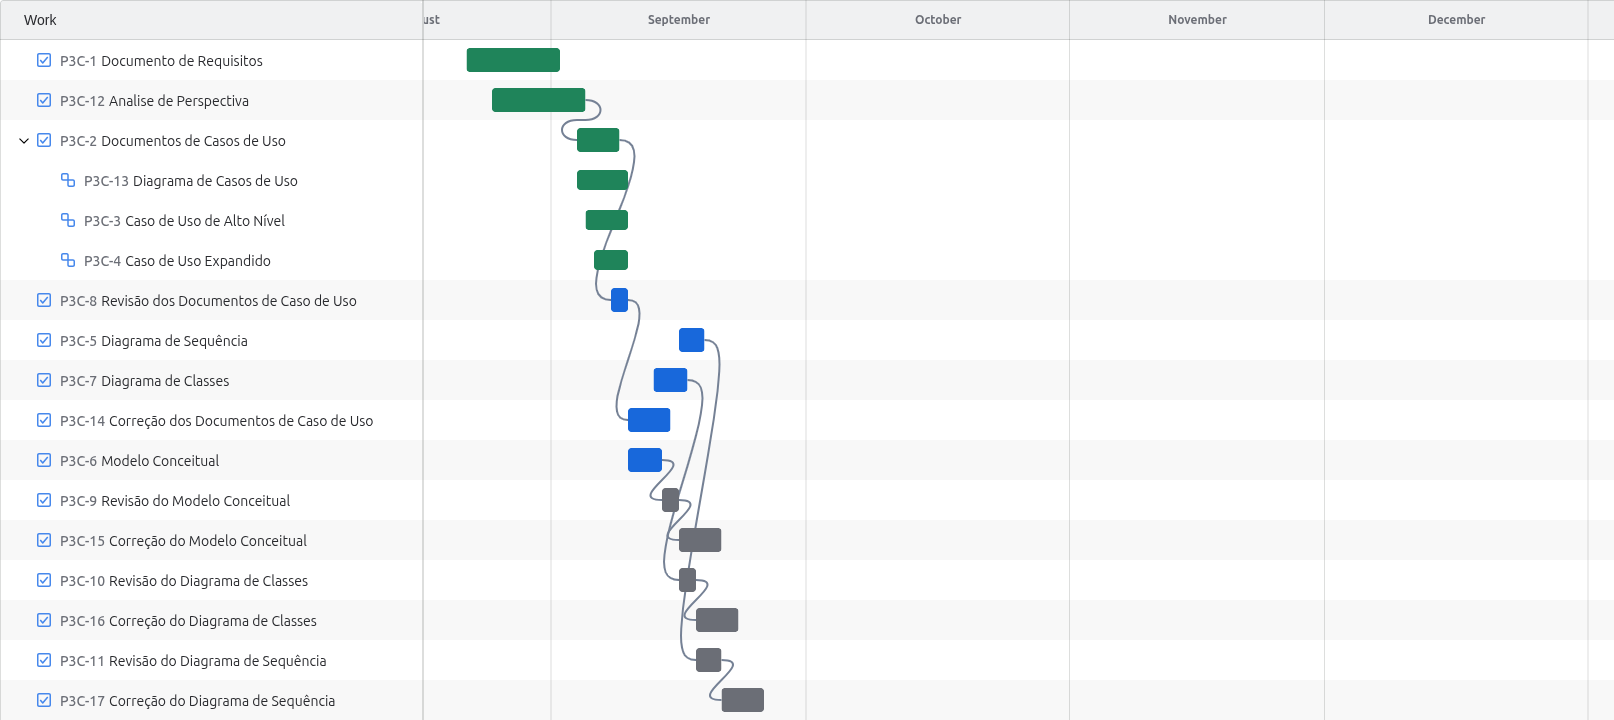
\includegraphics[width=\textwidth]{images/projeto_3___churrasco_2025-10-01_04.09pm.png}
    \caption{Gráfico de Gantt do Projeto - Sistema de Gestão de Churrascos Entre Amigos}
    \label{fig:gantt_chart}
\end{figure}

O gráfico de Gantt ilustra claramente:
\begin{itemize}
    \item A sequência temporal de todas as atividades
    \item As dependências críticas entre tarefas
    \item A alocação de recursos por equipe ao longo do tempo
    \item Os marcos principais de cada sprint
    \item O caminho crítico do projeto
\end{itemize}

\subsubsection{Caminho Crítico}
\textbf{Sequência do Caminho Crítico:} 1.1 → 1.2 → 1.3 → 1.4 → 2.1 → 2.1.1 → 2.1.2 → 2.1.3 → 2.2 → 2.3 → 2.4 → 3.1 → 3.2 → 3.3 → 4.1 → 4.2 → 4.3 → 4.4

Como o cronograma é totalmente sequencial, \textbf{todas as tarefas fazem parte do caminho crítico}. Qualquer atraso em uma tarefa atrasa o projeto inteiro.

\subsection{Marcos Principais}
\begin{itemize}
    \item \textbf{M0 (Fim do Sprint 0):} Documentação completa e aprovada - Dia 27
    \item \textbf{M1 (Fim do Sprint 1):} Módulo de cadastros funcionando - Dia 53
    \item \textbf{M2 (Fim do Sprint 2):} Sistema financeiro implementado - Dia 76
    \item \textbf{M3 (Fim do Sprint 3):} Sistema completo e entregue - Dia 86
\end{itemize}

\subsection{Entregáveis por Sprint}
\begin{itemize}
    \item \textbf{Sprint 0:} Documento de Requisitos, Casos de Uso, Diagramas UML
    \item \textbf{Sprint 1:} Módulo de cadastros funcionando, Diagramas de Colaboração
    \item \textbf{Sprint 2:} Sistema financeiro completo, Módulo de despesas
    \item \textbf{Sprint 3:} Sistema integrado, testado e documentado
\end{itemize}

\subsection{Critérios de Aceitação}
Cada marco deve atender aos seguintes critérios:
\begin{itemize}
    \item Todos os entregáveis foram revisados e aprovados pela equipe SQA
    \item Cobertura de testes mínima de 80\% para código
    \item Documentação atualizada e revisada
    \item Aprovação formal dos gerentes de projeto
\end{itemize}

\section{Organização da Equipe}

\subsection{Estrutura da Disciplina}

O projeto está inserido no contexto da disciplina de Engenharia de Software 2, onde cada dupla de alunos assume diferentes papéis em múltiplos projetos, proporcionando experiência completa no ciclo de desenvolvimento de software.

\subsection{Estrutura da Equipe para Este Projeto}

Para o \textbf{Projeto 3 - Sistema de Gestão de Churrascos Entre Amigos}, a estrutura da equipe segue o modelo de papéis rotacionados conforme especificado:

\begin{itemize}
    \item \textbf{Gerentes (G) - Julio, Ricardo, Igor:} 
    \begin{itemize}
        \item Planejamento estratégico e operacional
        \item Controle de cronograma e recursos
        \item Coordenação entre equipes das outras duplas
        \item Tomada de decisões de alto nível
        \item Comunicação com stakeholders e professor
        \item Criação e manutenção deste Plano de Projeto
        \item Monitoramento de riscos e qualidade
        \item Aprovação de entregáveis e marcos
    \end{itemize}
    
    \item \textbf{SQA - Garantia da Qualidade (Luiz e Sara):}
    \begin{itemize}
        \item Elaboração de planos de teste
        \item Execução de testes funcionais e não-funcionais
        \item Identificação e documentação de defeitos
        \item Revisão de artefatos de projeto
        \item Validação da qualidade final do produto
        \item Definição de critérios de aceitação
        \item Auditoria de processos de desenvolvimento
        \item Relatórios de qualidade e métricas
    \end{itemize}
    
    \item \textbf{A\&P - Analistas e Programadores (Augusto e Coleta):}
    \begin{itemize}
        \item Análise e especificação de requisitos
        \item Modelagem conceitual e de dados
        \item Design de arquitetura do sistema
        \item Criação de diagramas UML
        \item Validação de especificações
        \item Prototipação de interfaces
        \item Documentação técnica de análise
        \item Suporte ao design de banco de dados
    \end{itemize}
    
    \item \textbf{COD - Programadores (Guilherme Carrara e Guilherme Digiorgi):}
    \begin{itemize}
        \item Implementação das funcionalidades
        \item Codificação seguindo padrões estabelecidos
        \item Integração de módulos
        \item Correção de bugs e melhorias
        \item Documentação técnica do código
        \item Testes unitários básicos
        \item Configuração de ambiente de desenvolvimento
        \item Versionamento e controle de código
    \end{itemize}
\end{itemize}

\subsection{Matriz de Responsabilidades}

\begin{longtable}{|p{4cm}|c|c|c|c|}
\hline
\textbf{Atividade} & \textbf{Gerentes} & \textbf{SQA} & \textbf{A\&P} & \textbf{COD} \\
\hline
Planejamento & R & C & C & C \\
\hline
Análise de Requisitos & A & R & R & C \\
\hline
Design do Sistema & A & R & R & C \\
\hline
Codificação & A & C & C & R \\
\hline
Testes & A & R & C & C \\
\hline
Documentação & R & R & R & R \\
\hline
Integração & A & R & C & R \\
\hline
Entrega & R & A & C & C \\
\hline
\end{longtable}

\textbf{Legenda:} R = Responsável, A = Aprovador, C = Consultado

\subsection{Alocação por Sprint}

\subsubsection{Sprint 0 - Preparação}
\begin{itemize}
    \item \textbf{Gerentes (Julio, Ricardo e Igor):} Planejamento inicial e definição de diretrizes
    \item \textbf{A\&P (Augusto e Coleta):} Foco principal - documentação e modelagem
    \item \textbf{COD (Guilherme Carrara e Guilherme Digiorgi):} Preparação do ambiente de desenvolvimento
    \item \textbf{SQA (Luiz e Sara):} Planejamento de estratégias de teste e qualidade
\end{itemize}

\subsubsection{Sprint 1 - Desenvolvimento Inicial}
\begin{itemize}
    \item \textbf{Gerentes (Julio, Ricardo e Igor):} Acompanhamento e controle do cronograma
    \item \textbf{A\&P (Augusto e Coleta):} Finalização de diagramas de colaboração
    \item \textbf{COD (Guilherme Carrara e Guilherme Digiorgi):} Foco principal - codificação de cadastros
    \item \textbf{SQA (Luiz e Sara):} Testes e revisão do módulo de cadastro
\end{itemize}

\subsubsection{Sprint 2 - Desenvolvimento Avançado}
\begin{itemize}
    \item \textbf{Gerentes (Julio, Ricardo e Igor):} Monitoramento de riscos e ajustes no plano
    \item \textbf{A\&P (Augusto e Coleta):} Suporte à codificação complexa
    \item \textbf{COD (Guilherme Carrara e Guilherme Digiorgi):} Foco principal - sistema financeiro e cálculos
    \item \textbf{SQA (Luiz e Sara):} Testes extensivos do sistema financeiro
\end{itemize}

\subsubsection{Sprint 3 - Finalização}
\begin{itemize}
    \item \textbf{Gerentes (Julio, Ricardo e Igor):} Preparação da entrega e documentação final
    \item \textbf{A\&P (Augusto e Coleta):} Revisão final e documentação
    \item \textbf{COD (Guilherme Carrara e Guilherme Digiorgi):} Correção de bugs e refinamentos
    \item \textbf{SQA (Luiz e Sara):} Testes finais e validação completa do sistema
\end{itemize}

\subsection{Comunicação e Coordenação}

\subsubsection{Reuniões Regulares}
\begin{itemize}
    \item \textbf{Daily Standups:} Reuniões diárias de 15 minutos entre as duplas
    \item \textbf{Sprint Planning:} Planejamento detalhado no início de cada sprint
    \item \textbf{Sprint Review:} Avaliação dos resultados ao final de cada sprint
    \item \textbf{Retrospectivas:} Identificação de melhorias no processo
    \item \textbf{Reuniões Interdisciplinares:} Coordenação com outros projetos da disciplina
\end{itemize}

\subsubsection{Ferramentas de Gestão}
\begin{itemize}
    \item Sistema de controle de versão (Git)
    \item Ferramenta de gestão de projetos (ex: Jira, Trello)
    \item Plataforma de comunicação (ex: Slack, Teams, WhatsApp)
    \item Repositório de documentação centralizado
    \item Ambiente de desenvolvimento compartilhado
\end{itemize}

\subsection{Relatórios de Gestão}

\subsubsection{Estrutura de Reportes}

O projeto seguirá uma estrutura hierárquica de reportes para garantir comunicação eficaz e controle adequado:

\begin{itemize}
    \item \textbf{Relatórios Diários:} Status updates das tarefas em andamento
    \item \textbf{Relatórios Semanais:} Progresso detalhado por sprint e identificação de impedimentos
    \item \textbf{Relatórios de Marco:} Avaliação completa ao final de cada sprint
    \item \textbf{Relatórios de Exceção:} Comunicação imediata de problemas críticos
\end{itemize}

\subsubsection{Métricas de Acompanhamento}

\begin{enumerate}
    \item \textbf{Progresso de Cronograma:}
    \begin{itemize}
        \item Percentual de tarefas concluídas no prazo
        \item Variação entre estimado vs realizado
        \item Identificação de gargalos
    \end{itemize}
    
    \item \textbf{Qualidade:}
    \begin{itemize}
        \item Número de defeitos por módulo
        \item Taxa de retrabalho
        \item Cobertura de testes
    \end{itemize}
    
    \item \textbf{Recursos:}
    \begin{itemize}
        \item Utilização da equipe por perfil
        \item Disponibilidade vs demanda
        \item Identificação de sobrecarga
    \end{itemize}
\end{enumerate}

\subsection{Responsabilidades Específicas dos Gerentes}

Como líderes do Projeto 3, Julio, Ricardo e Igor têm as seguintes responsabilidades adicionais:

\begin{itemize}
    \item Coordenar atividades com as outras duplas envolvidas no projeto
    \item Reportar progresso para o professor da disciplina
    \item Gerenciar dependências entre projetos da disciplina
    \item Assegurar qualidade e cumprimento de prazos
    \item Facilitar comunicação entre diferentes perfis
    \item Tomar decisões estratégicas quando necessário
    \item Manter documentação atualizada e acessível
    \item Resolver conflitos e impedimentos
    \item Aprovar mudanças de escopo ou cronograma
\end{itemize}

\subsection{Critérios de Qualidade e Entrega}

\begin{itemize}
    \item \textbf{Código:} Seguir padrões de codificação definidos, comentários adequados, versionamento correto
    \item \textbf{Documentação:} Completa, atualizada e revisada por pelo menos dois membros da equipe
    \item \textbf{Testes:} Cobertura mínima de 80\%, testes automatizados onde possível
    \item \textbf{Integração:} Builds automatizados sem falhas, integração contínua funcional
\end{itemize}


\end{document}
